\section{Diskussion og lyttetest}

\subsection{Lyttetest}
Da god lyd, eller bedre lyd er en objektiv holdning, har gruppen valgt at lave en lyttetest. I denne lyttetest, vil resultatet give os en indikation, om Jazz konfig, og Rock konfig, har den ønskede effekt. Testen er lavet på 13 personer. Grundet tidspres, er testen lavet som en udvidet "kan-du-høreforskel" \ test, hvor testpersonerne blot skal give indikation om hvilken afspilning der er bedst. Dette betyder også at middelværdi og spredning ikke kan findes på testen. Testen er derfor en test af trends, altså af hvad der lyder bedst. Herunder vil der beskrives en gennemgang af testen, og under bilag på  \autoref{fig:Lyttetest} kan den test ses, som blev udleveret til hver af test deltagerne.  
 
\subsubsection{Selve lyttetesten}
Testen er udført som en AB test, hvor der er tilføjet et C (ABC test), dette betyder at testpersonerne hører 3 konfigurationer af hver musikklip, hvorefter testpersonen skal vælge hvilken af de 3 konfigurationer som er bedst. Deltagerne kommer skiftevis ind i lytterummet, en af gangen, og bliver præsenteret for de 3 genrer. For at undgå bias i testen, er der valgt en version A og B, som har hver deres rækkefølge. lydniveauet for alle deltagerne er ens, og der er ikke taget højde for hverken alder eller køn.    

\subsubsection{Programmateriale}
De tre sange er som følge: \\
Jazz: Max Roach \& Abbey Lincoln - Lonesome Lover \\
Rock: ACDC - Thunderstruck \\
Pop: Taylor Swift - 22 \\
Disse sange er valgt ud fra, at de er forholdsvis kendte, og rammer deres genrer. Hver af sangene er klippet, så det varer 15 sekunder et sted i sangen omkring omkvædet. 

\subsubsection{Resultat}
På \autoref{fig:lytteresultat} ses resultatet af testen. Her ses flere forskellige tendenser:  \\Jazz musikken har ingen klare tendenser, dette betyder at vores Jazz konfiguration ikke har haft den ønskede virkning, som var at optimere/forbedre lyden til Jazz musik. \\Rock musikken har en klar tendens, nemlig at 8 ud af 13 testpersoner (61\%) foretrækker Rock konfigurationen ift. de to andre. Herved ses at Rock konfigurationen har den positive trend at forbedre lyden til Rock musik, som var målet for med denne konfiguration. \\
Pop musikken var taget med for at teste om det optimerede  standart filter var bedst, når ingen af de to musikgenrer, som var lavet forbedringer på, optrådte. Her ses igen en tendens, som indikerer at vores optimerede standart filter viser den største trend indenfor pop. 
 
\begin{figure}[H] 
	\center
	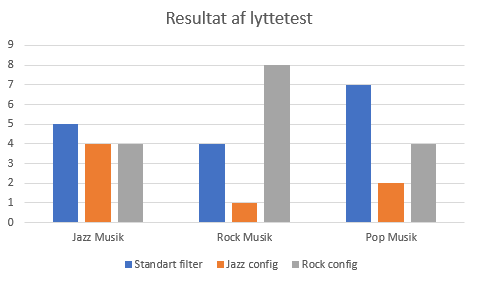
\includegraphics[width=0.8\linewidth]{figur/lytteresultat}\quad
	\caption{Resultat af lyttetesten}
	\label{fig:lytteresultat}
\end{figure}
Samlet set er projektgruppen tilfreds med resultatet, da Rock konfigurationen er den mest populære ved rock nummeret. Derudover er det optimerede standart filter populær blandt alle genrer, hvilket også er tilfredsstillende ift. projektgruppen, da standart filteret skulle passe til alt musik. På den negative side, vurderes jazz konfigurationen ikke til at leve op til de forventninger projektgruppen havde til konfigurationen, da det netop ikke er den mest populære konfiguration ved jazz musik.  


\subsection{Diskussion}
Igennem processen af produktet, mødte gruppen flere udfordringer. Da projektet omhandler højtalere som gruppen ingen data havde på, kom der problemstillinger ift. målinger. Den første udfordring kom herved, at ved måling af frekvensresponsen, blev afstanden mellem højtaler og mikrofon lavet ud fra afstandsmåling med tomstok. For at sikre at hver måling var ens, skulle gruppen have lavet en opstilling som altid stod ens. Hertil blev nogle af målingerne lidt forskellige, da opstillingen ikke var 100\% ens. Det hjalp heller ikke yderlig, at begge diskantenheder sidder forskudt et par centimeter til venstre ift. basenhederne, hvilket gjorde det besværligt at placere mikrofonen præcist lige langt mellem enhederne. Dette var en af ulemperne ved at købe et gammelt kabinet, hvor der netop allerede var boret huller til enhederne, som derfor ikke kunne placeres helt som ønsket. 


Gennem optimeringsfasen forsøgte gruppen af lave frekvensresponsen så flad som muligt. Efter målingen af diskanten og basenheden, valgte gruppen at lave et dele filter ved 4 kHz og hertil et optimeret filter. Dette gav et stort set fladt frekvensrespons, da højtalerne blev placeret i kabinettet, som det ses på  \autoref{fig:Optimering-forskel}. Der dog kom et lille dyk ved omkring 7kHz på frekvensreposen, som kan skyldes en destruktiv interferens på grund af stående bølger inde i kabinettet eller andre kabinet resonanser. Men ellers blev frekvensresponsen af den optimerede konfiguration (config 2) som forventet og tilfredsstillende. 

Ideen bag de to konfigurationer var, at forstærke og dæmpe bestemte frekvenser ift. hvilke instrumenter som indgår i musikgenren. Dette gav dog den problemstilling, at ved at ændre forstærkningsforholdene af frekvenserne på baggrund af et bestemt instrument, muligvis forstærkede negative effekter for andre instrumenter. Dette er også grunden til at man normalt i et lydstudie retter hvert instrument til, for at få det bedste fra hvert instrument. Ud fra lyttetesten, ses at de negative effekter ved jazz konfigurationen, kan være årsag til den ikke er at foretrække. Modsat ses ved rock konfigurationen, at de tilsigtede effekter har en virkning på lydoplevelsen. 

Lyttetesten er lavet for at verificere nogle af de pointer og tiltag som de to konfigurationer er lavet ud fra. Hvis gruppen havde haft mere tid, og flere forsøgspersoner, ville fokus rettes på at lave en test ud fra nogle subjektive parametre. Her kunne parametre som fullness og crispness være nogle af de parametre, som kunne testes. Hertil ville der også kunne laves en skala, så man kunne beregne middelværdi og spredning på resultaterne. Herefter kunne man bruge data/infomationerne til at finpudse de to konfigurationer, så de begge gav den bedste lytte oplevelse til begge musik genre.
\\ En anden vinkel, gruppen kunne have sat i fokus, var at repetere den samme sekvens af de 3 lydklip, for at se om besvarelser var tilfældige eller deterministiske. Herudover kunne man også tilføje flere musik numre, af samme genrer, for at verificere, at resultatet er gængs over forskellige numre. 

      
